\documentclass[11pt]{article}
\usepackage[paperwidth=254mm,paperheight=142.875mm,margin=12mm]{geometry}
\usepackage{amsmath,amssymb}
\usepackage{graphicx}

\newcommand{\R}{\mathbb{R}}

\begin{document}

\begin{center}
{\LARGE\bfseries Part I: Background notes}\par\vspace{4pt}
{\large Supporting material for understanding the paper. Not presented.}
\end{center}
\vspace{6pt}\hrule\vspace{10pt}

\section{Chain rule}

\paragraph{Setup.} Let $h:\R^n\to\R^m$ be one layer and $\ell:\R^m\to\R$ be everything after it (the rest of the network and the loss), so the loss is $L(x)=\ell\big(h(x)\big)$. The \emph{local Jacobian} of the layer is the $m\times n$ matrix
\[
J_h(x)=\frac{\partial h}{\partial x},\qquad (J_h)_{ij}=\frac{\partial h_i}{\partial x_j}.
\]

\paragraph{Chain rule.}
\[
\nabla_x L \;=\; J_h(x)^{\top}\,\nabla \ell\big(h(x)\big).
\]
Here $\nabla \ell\big(h(x)\big)$ is the \emph{downstream gradient} (what the rest of the network wants the layer's output to do), and $J_h(x)^{\top}$ converts it into a gradient on the layer's input $x$.

\paragraph{Intuition.} The downstream gradient says how the loss would change if the layer's \emph{output} moved. The local Jacobian says how the layer's output moves when its \emph{input} $x$ moves. Multiplying the two gives how the loss changes when $x$ moves, which is what gradient descent needs to update $x$. Backpropagation repeats this layer by layer, so every layer's local Jacobian is a factor in the gradient that reaches earlier layers.

\paragraph{Two cases relevant to this paper.}
\begin{enumerate}
\item \textbf{Local Jacobian is zero}, $J_h(x)=0$. Then
\[
\nabla_x L = 0 \quad\text{for every downstream gradient}.
\]
\emph{Meaning:} small changes to $x$ do not change the layer's output, so the loss gives $x$ no direction to move. Gradient descent never updates $x$, and nothing before this layer learns either. This is what rounding (quantization) does.

\item \textbf{Local Jacobian is the identity}, $J_h(x)=I$. Then
\[
\nabla_x L = \nabla \ell\big(h(x)\big).
\]
\emph{Meaning:} the downstream gradient is passed back unchanged, as if the layer did nothing. Whatever the layer actually did to $x$ (for example, adding a rounding error) has no effect on the gradient, so earlier layers get no signal about it. This is what the Straight-Through Estimator (STE) assumes.
\end{enumerate}

\section{Ridge regression}

\paragraph{Why needed.} The paper's dequantizer $g$ is a ridge-regression fit of the original $x$ from the rounded $q$ (with $u=q$, $v=x$ below).

\paragraph{Notation.} For $u,v\in\R^N$: $\bar u=\frac1N\sum_i u_i$, $\overline{uv}=\frac1N\sum_i u_iv_i$, $\operatorname{Var}_u=\overline{u^2}-\bar u^{2}$, $\operatorname{Cov}_{uv}=\overline{uv}-\bar u\,\bar v$, and $\mathbf 1$ is the all-ones vector.

\paragraph{Problem.} Fit $v\approx a\,u+c\mathbf 1$, penalizing only the slope:
\[
\min_{a,c}\ \frac{1}{2N}\|a\,u+c\mathbf 1-v\|^2+\frac{\lambda}{2}a^2,\qquad \lambda>0 .
\]
Setting derivatives to zero:
\[
c^*=\bar v-a^*\bar u,\qquad a^*=\frac{\operatorname{Cov}_{uv}}{\operatorname{Var}_u+\lambda}.
\]
Without intercept ($c=0$): $a^*=\dfrac{\overline{uv}}{\overline{u^2}+\lambda}$.

\paragraph{Fit.} The vector of the line's predictions at the data points:
\[
\text{fit}=a^*u+c^*\mathbf 1=a^*(u-\bar u\mathbf 1)+\bar v\mathbf 1 .
\]

\paragraph{Role of $\lambda$.} (i) \emph{Stability:} the denominator is at least $\lambda>0$, so no division by zero even if all $u_i$ are equal. (ii) \emph{Shrinkage:} as $\lambda\to\infty$, $a^*\to0$ and the fit becomes the mean $\bar v\mathbf 1$.

\section{Quantization}

\paragraph{In short.} We select a grid of integers, assign one integer to each of our real numbers (rescale, then round to the nearest), and then try to get our real numbers back from those integers. Only the integers (plus one $s_f$, $b_f$ per block) are stored; the recovery is approximate, and the gap is the rounding error. The paper keeps the first two steps and changes only the last one: how to get back from the integers to the best possible real numbers.

\paragraph{Setup.} A block $x\in\R^N$ (weights or activations) is mapped to a $k$-bit integer grid $\{q_{\min},\dots,q_{\max}\}$ with $2^k$ levels. Notation A$a$W$w$: $a$-bit activations, $w$-bit weights.

\paragraph{Step 1: prequantization $f$.} Rescale $x$ onto the grid's range.
\begin{itemize}
\item Linear (centred data, e.g.\ weights): $f(x)=\dfrac{x}{s_f}$,\quad $s_f=\dfrac{\max_i|x_i|}{q_{\max}}$.
\item Affine (uncentred data, e.g.\ ReLU activations): $f(x)=\dfrac{x-b_f\mathbf 1}{s_f}$,\quad $s_f=\dfrac{x_{\max}-x_{\min}}{q_{\max}-q_{\min}}$,\quad $b_f=x_{\min}-s_f\,q_{\min}$.
\end{itemize}

\paragraph{Step 2: rounding and the error.} $\operatorname{round}$ is nearest integer, entrywise.
\[
q=\operatorname{round}\big(f(x)\big)=f(x)+\delta,\qquad \delta=\operatorname{round}\big(f(x)\big)-f(x),\qquad |\delta_i|\le\tfrac12 .
\]

\paragraph{Step 3: standard dequantization.} Undo the rescaling ($b_f=0$ in the linear case):
\[
\hat x=s_f\,q+b_f\mathbf 1=x+s_f\,\delta .
\]
Quantization is therefore $x$ plus an additive error of size at most $s_f/2$ per entry; fewer bits means larger $s_f$, hence larger error.

\section{The problem: zero gradient and the Straight-Through Estimator}

\paragraph{The chain during training.} The network stores the real $x$; the next layer uses the quantized-then-dequantized $\hat x$:
\[
x\ \xrightarrow{\ f\ }\ f(x)\ \xrightarrow{\ \operatorname{round}\ }\ q\ \xrightarrow{\ s_f q+b_f\mathbf 1\ }\ \hat x\ \longrightarrow\ \text{rest of network}\ \longrightarrow\ L,
\]
where
\begin{itemize}
\item $f(x)=\dfrac{x-b_f\mathbf 1}{s_f}$ rescales $x$ onto the integer grid ($b_f=0$ in the linear case); $s_f$ is the step size of the grid in real units, $b_f$ the real value of integer $0$;
\item $q=\operatorname{round}\big(f(x)\big)=f(x)+\delta$ is the stored integer vector, $\delta$ the rounding error, $|\delta_i|\le\frac12$;
\item $\hat x=s_f\,q+b_f\mathbf 1=x+s_f\,\delta$ is $x$ as seen after quantization.
\end{itemize}

\paragraph{Chain rule.} Gradient descent needs $\nabla_x L$:
\[
\nabla_x L=\Big(\frac{\partial \hat x}{\partial x}\Big)^{\!\top}\nabla_{\hat x}L,
\qquad
\frac{\partial \hat x}{\partial x}
=\underbrace{s_f}_{\text{scale back}}\cdot\underbrace{\frac{\partial q}{\partial f(x)}}_{\text{round}}\cdot\underbrace{\frac{1}{s_f}}_{f}
=\frac{\partial q}{\partial f(x)} .
\]
The two scalings cancel, so the local gradient is exactly the slope of $\operatorname{round}$.

\paragraph{Zero gradient.} $\operatorname{round}$ is a staircase: $\frac{d}{du}\operatorname{round}(u)=0$ for $u\notin\mathbb Z+\frac12$ (undefined at half-integers). Hence $\frac{\partial q}{\partial f(x)}=0$ almost everywhere and $\nabla_x L=0$: $x$ and all earlier layers never update (case 1 of Section 1).

\paragraph{STE (Bengio et al., 2013).} Treat the rounding error as a constant in the backward pass:
\[
q=f(x)+\delta,\qquad \delta=\operatorname{stopgrad}\big(\operatorname{round}(f(x))-f(x)\big).
\]
Forward: $q=\operatorname{round}(f(x))$ exactly. Backward: $\frac{\partial q}{\partial f(x)}=I$, so $\frac{\partial \hat x}{\partial x}=I$ and $\nabla_x L=\nabla_{\hat x}L$ (case 2 of Section 1).

\paragraph{The blind spot.}
\[
\text{forward: }\ \hat x=x+s_f\,\delta,\qquad\qquad \text{backward: }\ \frac{\partial \hat x}{\partial x}=I .
\]
The forward pass is changed by the error, but the local Jacobian is the same as with no quantization at all; $\delta$ does not appear in it. Earlier layers get no signal about how their rounding error hurts the loss, so they cannot learn to be robust to it. At 1--2 bits $s_f\delta$ is large and STE training becomes unstable. ($\delta$ still affects \emph{where} $\nabla_{\hat x}L$ is evaluated; it is absent only from the local factor $\partial\hat x/\partial x$, which is the factor the paper changes.)

%==============================================================
% SLIDES: one slide per page
%==============================================================
\clearpage
\vspace*{\fill}
\begin{center}
{\Huge\bfseries Part II: Slides}\par\vspace{10pt}
\end{center}
\vspace*{\fill}
\newcommand{\slide}[1]{\clearpage\noindent{\Large\bfseries #1}\par\vspace{4pt}\hrule\vspace{10pt}}

% TITLE SLIDE
\clearpage
\vspace*{\fill}
\begin{center}
{\LARGE\bfseries Robust Training of Neural Networks\\[4pt] at Arbitrary Precision and Sparsity}\par\vspace{8pt}
{\large C.~Ye, G.~Chu, Y.~Liu, Y.~Zhang, L.~Lew, L.~Zhang, M.~Sandler, A.~Howard}\par
{\large Google DeepMind \quad\textbullet\quad ICLR 2026}\par\vspace{28pt}
{\large Presented by}\par\vspace{6pt}
{\Large Ayush Srivastava (2026AIB2015)\qquad Sarvesh Nikas (2026AIB2045)}
\end{center}
\vspace*{\fill}

\slide{Why quantization, and the forward pass during training}

\paragraph{Why quantization.} Modern neural networks are huge: a language model has billions of weights, each stored as a 32-bit or 16-bit floating-point number. This makes models too big to fit on a phone, slower to run, and costly in energy. Quantization stores each weight with far fewer bits: 4, 2 or 1 bit instead of 16 or 32.

\paragraph{Training with quantization.} During training the network keeps the float weights $x$ and updates them by gradient descent. We could compute with $x$, but we deliberately use the quantized version $\hat x$ in the forward pass, so the network learns to be robust to the rounding it will face at inference. After training, $x$ is discarded; only the low-bit integers $q$ (plus one $s_f$, $b_f$ per block) are kept.

\paragraph{The forward pass during training.}
\[
x\ \xrightarrow{\ f\ }\ f(x)\ \xrightarrow{\ \operatorname{round}\ }\ q\ \xrightarrow{\ s_f q+b_f\mathbf 1\ }\ \hat x\ \longrightarrow\ \text{rest of network}\ \longrightarrow\ L
\]
\begin{itemize}
\item $x\in\R^N$: float block, kept and updated during training.
\item $f(x)=\dfrac{x-b_f\mathbf 1}{s_f}$: rescales $x$ onto the $k$-bit integer grid; $s_f$ = grid step in real units, $b_f$ = real value of integer $0$ ($b_f=0$ in the linear case).
\item $q=\operatorname{round}\big(f(x)\big)=f(x)+\delta$: the integers, with rounding error $|\delta_i|\le\frac12$.
\item $\hat x=s_f\,q+b_f\mathbf 1=x+s_f\,\delta$: $x$ as seen after quantization; this is what the next layer uses.
\end{itemize}

\slide{The problem: the true gradient is zero}

\paragraph{Chain rule through the quantizer.} Gradient descent needs $\nabla_x L$:
\[
\nabla_x L=\Big(\frac{\partial \hat x}{\partial x}\Big)^{\!\top}\nabla_{\hat x}L,
\qquad
\frac{\partial \hat x}{\partial x}
=\underbrace{s_f}_{\text{scale back}}\cdot\underbrace{\frac{\partial q}{\partial f(x)}}_{\text{round}}\cdot\underbrace{\frac{1}{s_f}}_{f}
=\frac{\partial q}{\partial f(x)} .
\]
The two scalings cancel: the local gradient is exactly the slope of $\operatorname{round}$.

\paragraph{Round is a staircase.}
\[
\frac{d}{du}\operatorname{round}(u)=0\quad\text{for } u\notin\mathbb Z+\tfrac12,\qquad\text{undefined at } u\in\mathbb Z+\tfrac12 .
\]
Hence $\dfrac{\partial q}{\partial f(x)}=0$ almost everywhere, so
\[
\nabla_x L=0 .
\]

\paragraph{Consequence.} A small change in $x$ does not change $q$, so the loss gives $x$ no direction to move: $x$ and every layer before it never update. Training cannot start.

\slide{The standard fix: Straight-Through Estimator (STE)}

\paragraph{Idea.} Forward pass: round exactly as before. Backward pass: pass the gradient straight through the rounding, i.e.\ replace the true slope of $\operatorname{round}$ (zero) by $1$. This is a chosen rule, not a derived derivative.

\paragraph{Decomposition.} Write the rounded value as the smooth part plus the rounding error:
\[
q=\operatorname{round}\big(f(x)\big)=f(x)+\delta,
\qquad
\delta=\operatorname{stopgrad}\Big(\operatorname{round}\big(f(x)\big)-f(x)\Big),
\]
where $\operatorname{stopgrad}$ means: same value in the forward pass, treated as a constant (zero derivative) in the backward pass.

\paragraph{Forward.} $f(x)+\delta=\operatorname{round}\big(f(x)\big)$ exactly, so the network still sees quantized values.

\paragraph{Backward.} $\delta$ is a constant, so
\[
\frac{\partial q}{\partial f(x)}=\frac{\partial f(x)}{\partial f(x)}+\underbrace{\frac{\partial \delta}{\partial f(x)}}_{=\,0}=I .
\]
Substituting into the chain rule of the previous slide,
\[
\frac{\partial \hat x}{\partial x}=s_f\cdot I\cdot\frac{1}{s_f}=I,
\qquad\text{hence}\qquad
\nabla_x L=\nabla_{\hat x}L .
\]

\paragraph{Effect.} The gradient reaching $x$ is no longer zero, so $x$ and earlier layers update and training works.

\vfill
\noindent{\small\textit{Reference:} Y.~Bengio, N.~L\'eonard, A.~Courville, ``Estimating or propagating gradients through stochastic neurons for conditional computation,'' arXiv:1308.3432, 2013.}

\slide{Why STE fails: the blind spot}

\paragraph{Forward and backward disagree.}
\[
\text{forward: }\ \hat x=x+s_f\,\delta,
\qquad\qquad
\text{backward: }\ \frac{\partial \hat x}{\partial x}=I .
\]
\begin{itemize}
\item The forward pass uses the rounded values: every entry is shifted by its rounding error $s_f\delta_i$, which changes the output and the loss.
\item The local Jacobian is $I$: exactly what it would be with no quantization at all ($\hat x=x$). $\delta$ does not appear in it.
\item So earlier layers get no signal about how rounding hurts the loss, and cannot learn to be robust to it. The paper calls $\delta$ a ``ghost of departed quantities'' (Berkeley, 1754).
\item At 8 bits $s_f\delta$ is tiny and ignoring it is harmless. At 1--2 bits it is as large as the values themselves: the gradient no longer matches what the forward pass did, and training becomes unstable (STE diverges at A1W1, next slide, left).
\item With affine quantization, STE barely learns the offset: no gain over linear (next slide, right).
\end{itemize}

\slide{STE at 1 bit: results from the paper}

\noindent
\begin{minipage}[t]{0.49\textwidth}\centering
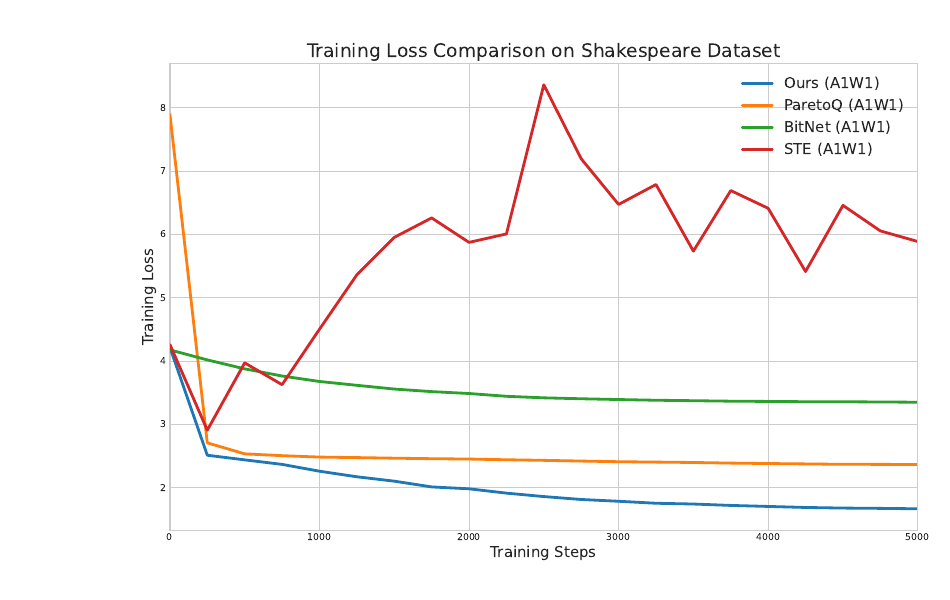
\includegraphics[width=\linewidth]{figs/fig1a_ste_divergence.png}\\[4pt]
\small Training loss, 1-bit weights and activations (A1W1), small GPT on Shakespeare. STE (red) diverges; the paper's method (blue) converges.
\end{minipage}\hfill
\begin{minipage}[t]{0.49\textwidth}\centering
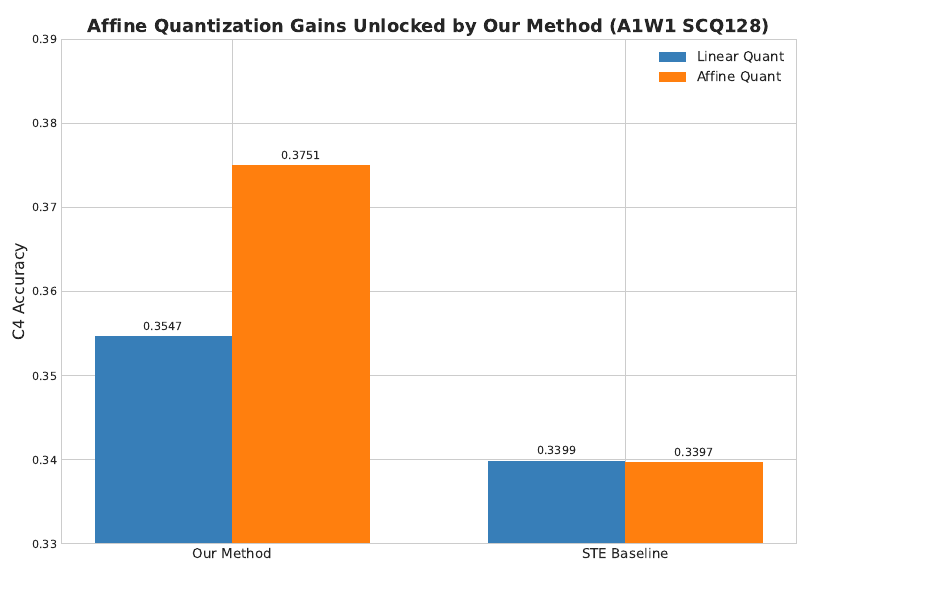
\includegraphics[width=\linewidth]{figs/fig1b_affine.png}\\[4pt]
\small Accuracy at A1W1, linear vs.\ affine quantization. Under STE affine gives no gain; with the paper's method it does.
\end{minipage}

\vfill
\noindent{\small\textit{Source:} Ye et al., ``Robust Training of Neural Networks at Arbitrary Precision and Sparsity,'' ICLR 2026, Fig.~1.}

\slide{Toy implementation}

\paragraph{Model.} A small character-level GPT (decoder-only transformer): 4 blocks, 4 attention heads, embedding size 128, context of 64 characters, 0.82M parameters. Built following Karpathy's ``Let's build GPT: from scratch'' and nanoGPT, the same family as the paper's nanoGPT Shakespeare experiment.

\paragraph{Data.} Tiny Shakespeare: 1.1M characters, 65-character vocabulary, first 90\% for training, last 10\% for validation. Task: predict the next character.

\paragraph{Quantization.} All linear layers inside the transformer blocks, weights and input activations, $k$ bits (A$k$W$k$), affine, one $s_f$, $b_f$ per row. Embeddings and the output layer stay full precision.

\paragraph{Runs.} Same seed, AdamW (lr $10^{-3}$), batch 64, 3000 steps; only the dequantization step differs. Float (no quantization, baseline); STE, $\hat x=s_f\,q+b_f\mathbf 1$; ridge, $g(q)=s_g\,q+b_g\mathbf 1$ with $\lambda=0.01$. STE and ridge at $k=1,2,4$.

\vfill
\noindent{\small\textit{References:} A.~Karpathy, ``Let's build GPT: from scratch, in code, spelled out'' (2023) and nanoGPT, \texttt{github.com/karpathy/nanoGPT}; Tiny Shakespeare from \texttt{github.com/karpathy/char-rnn}.}

\slide{Toy implementation: results}

\noindent
\begin{minipage}[t]{0.49\textwidth}\centering
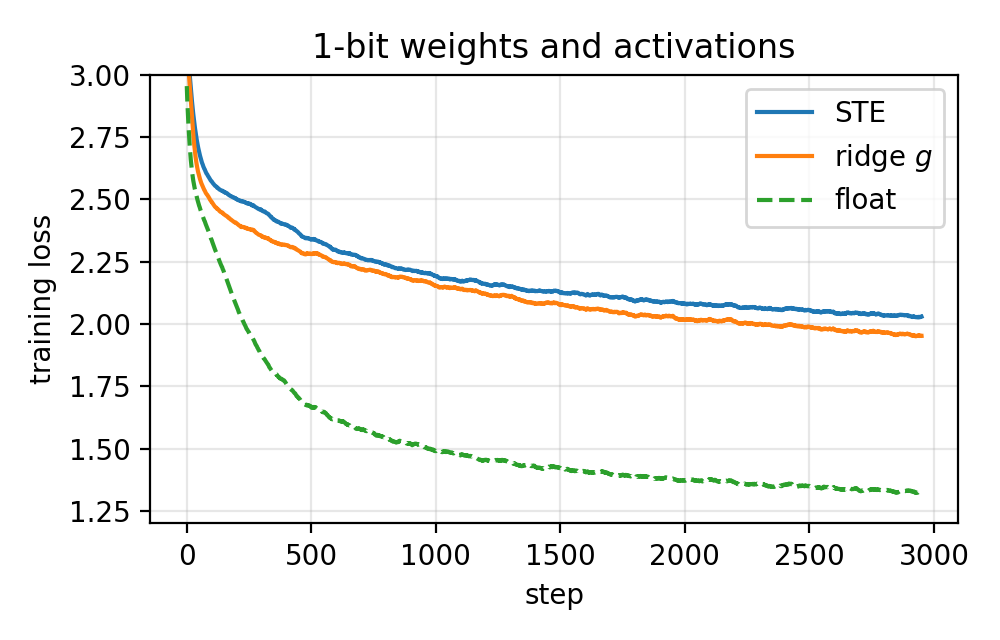
\includegraphics[width=0.85\linewidth]{implementation/plots/loss_k1.png}\\[4pt]
\small Training loss at A1W1 (smoothed over 50 steps).
\end{minipage}\hfill
\begin{minipage}[t]{0.49\textwidth}\centering
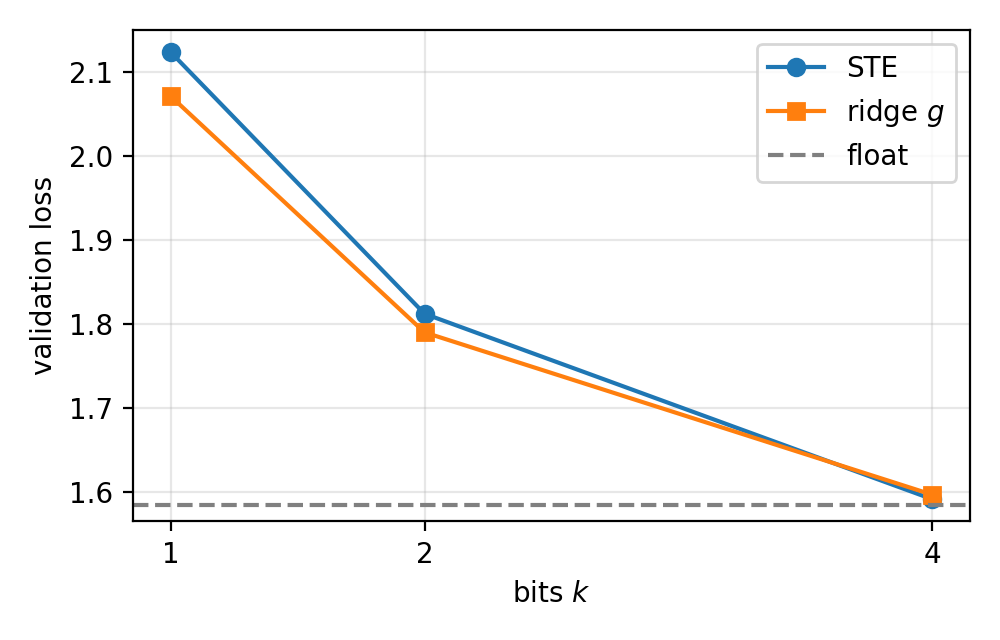
\includegraphics[width=0.85\linewidth]{implementation/plots/val_vs_bits.png}\\[4pt]
\small Final validation loss after 3000 steps.
\end{minipage}

\vspace{8pt}\noindent
\textbf{Gradient check} (1 bit, block of 64). Two inputs with the same $q$, rounding errors $\delta$ differing by up to 0.106, same upstream gradient:
\begin{center}\small
\begin{tabular}{lcc}
 & change in $\delta$ & change in gradient reaching $x$\\\hline
STE & 0.106 & 0.0000\\
ridge & 0.106 & 0.0144
\end{tabular}
\end{center}

\noindent\textbf{Size.} Float32 model 3.19 MB; at 1 bit 250 KB (12.7$\times$ smaller).

\end{document}
